% Preliminaries and Notation chapter
\chapter{Nozioni preliminari e notazione}
% Finite State Automata (+ related) section
\section{FSA non deterministici e deterministici}
Prima di introdurre le Choreography e i Choreographies Automata è necessario fare un breve richiamo di alcune nozioni fondamentali quali la nozione di Automa a Stati Finiti (FSA) e alcune operazioni possibili sugli stesssi.
Gli automi a stati finiti sono la descrizione di un sistema dinamico che si evolve nel tempo, esiste un parallelo tra gli automi e i calcolatori moderni, per esempio il flusso d'esecuzione di un programma può essere rappresentato attraverso un automa (come vedremo più avanti).
Alcune applicazioni pratiche di questi automi possono essere, per esempio, regular expression (RegEx o RegExp), lexer e parser ma possono anche essere impiegati, come vedremo in questa tesi, anche nel campo dei sistemi concorrenti.\\
Si noti che sebbene per gli scopi di questa tesi gli automi a stati finiti sono dei costrutti sufficentemente potenti esistono tuttavia altre classi di automi, espressivamente più potenti, ai quali corrispondo altrettante classi di linguaggi (si veda, per esempio, gli automi a pila) tuttavia gli automi appartenenti a questa classe sono tra i più semplici e immediati e forniscono una sufficente espressività per gli scopi di questa tesi.

\begin{definition}[Finite State Automata]
    Un automa a stati finiti (FSA) è una tupla A = $\langle \mathcal{S}, s_0, \mathcal{F}, \mathcal{L}, \delta \rangle$ dove:
    \begin{itemize}
        \item $\mathcal{S}$ è un insieme finito di stati
        \item $s_0 \in \mathcal{S}$ è lo stato iniziale dell'automa
        \item $\mathcal{F}$ è l'insieme degli stati finali (o di accettazione)
        \item $\mathcal{L}$ è l'alfabeto finito, talvolta detto anche insieme di label ($\epsilon \notin \mathcal{L}$)
        \item $\delta : \mathcal{S} \times (L \cup \{\epsilon\}) \rightarrow \mathcal{P}(\mathcal{S})$ è la funzione di transizione ($\epsilon$ denota la stringa vuota)
    \end{itemize}
\end{definition}

\begin{remark}
    Tipicamente è solito trovare anche una definizione alternativa ma equivalente in cui l'insieme degli stati di terminazione $\mathcal{F}$ non è presente, in tal caso assumiamo che ogni $s \in \mathcal{S}$ sia uno stato di accettazione.
\end{remark}

\begin{remark}
    Va notato anche che questa definizione coincide con quella di automa a stati finiti \emph{non deterministico}, solitamente indicato in letteratura con la sigla NFA (\emph{Non Deterministic Finite Automata}) e distinto dalla nozione di DFA (\emph{Deterministic Finite Automata}).
\end{remark}

\begin{definition}[Deterministic Finite Automata]
    Un automa a stati finiti deterministico è una tupla D = $\langle \mathcal{S}, s_0, \mathcal{F}, \mathcal{L}, \delta \rangle$ dove $\delta : \mathcal{S} \times L \rightarrow \mathcal{S}$
\end{definition}
Le varianti deterministiche si distinguono dalle loro controparti non deterministiche dal fatto che non ammettono ne l'utilizzo di $\epsilon$ transizioni, ne l'utilizzo di transizioni \emph{uscenti}, dallo stesso stato, con la medesima etichetta. Sebbene queste due varianti siano tra loro equivalenti, l'utilizzo di una variante rispetto all'altra può essere determinato da fattori come: necessità di una maggiore elasticità (gli NFA sono meno stringenti rispetto ai DFA) o di una migliore chiarezza (i DFA sono più immediati e semplici).\\
In ogni caso è sempre possibile, dato un NFA qualunque, ottenere un DFA ad esso equivalente. L'algoritmo che permette di fare questa trasformazione fa uso estensivo di \emph{$\epsilon$ closure} e della funione \emph{mossa} che andremo a definire di seguito:

\begin{definition}[$\epsilon$ closure]
    Fissato un NFA N = $\langle \mathcal{S}, s_0, \mathcal{F}, \mathcal{L}, \delta \rangle$ ed uno stato $s \in \mathcal{S}$ si dice $\epsilon$ closure di s, indicata con $\epsilon$-clos(s), il più piccolo $\mathcal{R} \subseteq \mathcal{S}$ tale che:
    \begin{itemize}
        \item $s \in \epsilon$-clos(s)
        \item se x $\in \epsilon$-clos(s) allora $\delta(x, \epsilon) \subseteq \epsilon$-clos(s)
    \end{itemize}
\end{definition}

\begin{remark}
    Se $\mathcal{X}$ è un insieme di stati definiamo $\epsilon$-clos($\mathcal{X}$) come $\bigcup_{x \in \mathcal{X}} \epsilon \mbox{-clos(x)}$.
\end{remark}

\begin{definition}[Mossa]
    Dato un insieme di stati $\mathcal{X} \subseteq \mathcal{S}$ e un simbolo $\alpha \in \mathcal{L}$ definiamo la funzione \emph{mossa}: $\mathcal{P(S)} \times \mathcal{L} \longrightarrow \mathcal{P(S)}$ tale che: \emph{mossa}$(\mathcal{X}, \alpha) = \bigcup_{x \in \mathcal{X}}(\delta(x, \alpha))$, , ovvero l'insieme di stati raggiungibili da un dato insieme di stati di partenza, leggendo in input $\alpha$.
\end{definition}
\newpage % ! Avoid forcefully break page
L'algoritmo che permette di ricavare un DFA da un qualsiasi NFA è il seguente:
\begin{algorithm}
    \caption{Costruzione per sottoinsiemi}\label{alg:cap}
    \begin{algorithmic}
        \State $x \gets$ $\epsilon$-clos($s_0$) \Comment{Lo stato iniziale del DFA}
        \State $\mathcal{T} \gets \{ x \}$                   \Comment{Un insieme di $\epsilon$-clos}
        \While{$\exists$ t $\in \mathcal{T}$ non marcato}
        \State marca(t)
        \ForEach {$\alpha \in \mathcal{L} $}
        \State $r \gets \epsilon$-clos(mossa(t, $\alpha$))
        \If {$r \notin \mathcal{T}$}
        \State $\mathcal{T} \gets \mathcal{T} \cup \{r\}$
        \EndIf
        \State $\delta(t, \alpha) \gets r$  \Comment{Denota che la $\delta$ del DFA con input t ed $\alpha$ darà output r}
        \EndFor
        \EndWhile
    \end{algorithmic}
\end{algorithm}\\
Si noti che $x$, $\mathcal{T}$ e $\delta$ saranno rispettivamente lo stato iniziale, l'insieme degli stati e la funzione di transizione del DFA corrispondente, $\mathcal{F}$ sarà invece l'insieme di tutti i $t \in \mathcal{T}$ che al loro interno contengono almeno uno stato finale dell'NFA di partenza mentre $\mathcal{L}$ rimane invariato. Quindi il DFA ottenuto in output sarà D = $\langle \mathcal{T}, x, \mathcal{F}, \mathcal{L}, \delta \rangle$.

\subsection{Esempi}
Per concludere questa sezione mostriamo di seguito un esempio dei vari concetti mostrati in questa sezione. Il seguente è un NFA N un grado di riconoscere la Regular Expression $(a|b)^*ba$:
\begin{figure}[ht]
    \centering
    \begin{tikzpicture}[->,>=stealth',node distance=2cm,scale=1, transform shape]
        \node[state,initial] (q0) {$q_0$};
        \node[state] (q1) [right of=q0] {$q_1$};
        \node[state] (q2) [above right of=q1] {$q_2$};
        \node[state] (q3) [right of=q2] {$q_3$};
        \node[state] (q4) [below right of=q1] {$q_4$};
        \node[state] (q5) [right of=q4] {$q_5$};
        \node[state] (q6) [above right of=q5] {$q_6$};
        \node[state] (q7) [right of=q6] {$q_7$};
        \node[state] (q8) [right of=q7] {$q_8$};
        \node[state, accepting] (q9) [right of=q8] {$q_9$};
        \draw
        (q0) edge[above] node{$\epsilon$} (q1)
        (q0) edge[bend left=60, above] node{$\epsilon$} (q7)
        (q1) edge[above] node{$\epsilon$} (q2)
        (q2) edge[above] node{$a$} (q3)
        (q3) edge[above] node{$\epsilon$} (q6)
        (q1) edge[above] node{$\epsilon$} (q4)
        (q4) edge[above] node{$b$} (q5)
        (q5) edge[above] node{$\epsilon$} (q6)
        (q6) edge[above] node{$\epsilon$} (q7)
        (q6) edge[above] node{$\epsilon$} (q1)
        (q7) edge[above] node{$b$} (q8)
        (q8) edge[above] node{$a$} (q9);
    \end{tikzpicture}
    \caption{Un possibile NFA che riconosce la RegEx $(a|b)^*ba$}
    \label{fig:NFA}
\end{figure}\\\\
Si noti che questo è solo un \emph{possibile} NFA in grado di riconscere il linguaggio dato ma ne esistono infiniti altri ad equivalenti ad esso. Vediamo ora invece il DFA D, equivalente ad N, calcolato tramite l'algorimo di \emph{Costruzione per sottoinsiemi}
\begin{figure}[ht]
    \centering
    \begin{tikzpicture}[->,>=stealth',shorten >=1pt,auto,node distance=3cm,scale=1, transform shape]
        \node[state,initial] (A) {$A$};
        \node[state] (B) [above right of=A] {$B$};
        \node[state] (C) [right of=A] {$C$};
        \node[state, accepting] (D) [above right of=C] {$D$};
        \draw
        (A) edge[above] node{$a$} (B)
        (A) edge[above] node{$b$} (C)
        (B) edge[loop above] node{$a$} (B)
        (B) edge[above] node{$b$} (C)
        (C) edge[loop below] node{$b$} (C)
        (C) edge[bend right, above] node{$a$} (D)
        (D) edge[above] node{$a$} (B)
        (D) edge[bend right,above] node{$b$} (C);
    \end{tikzpicture}
    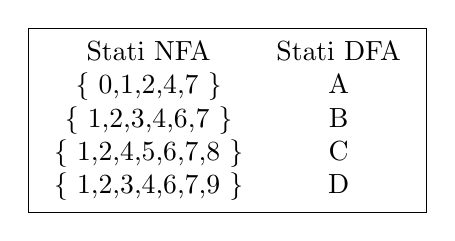
\begin{tikzpicture}
        \node (NFA to DFA) [shape=rectangle,draw] {
            \begin{tabular}{c c}
                Stati NFA           & Stati DFA \\
                \{ 0,1,2,4,7 \}     & A         \\
                \{ 1,2,3,4,6,7 \}   & B         \\
                \{ 1,2,4,5,6,7,8 \} & C         \\
                \{ 1,2,3,4,6,7,9 \} & D
            \end{tabular}
        };
    \end{tikzpicture}
    \caption{Il DFA equivalente a quello in figura 2.1}
    \label{fig:DFA}
\end{figure}

\section{Choreography Automata}
Passiamo ora alla definizione dei \emph{Choreography Automata} (CA); iniziamo diversificando la nozione di \emph{Choreographies} e \emph{Choreography Automata} il primo è un modello logico che permette di specificare le interazioni tra più attori (siano essi processi, programmi, etc.) all'interno di un sistema (concorrente nel nostro caso) mentre i secondi sono invece sono inece un'\emph{implementazione} possibile per questo modello. In questo caso noi stiamo scegliendo di implementare le Choreographies tramite degli Automi a Stati Finiti ma questo non esclude altre possibili implementazioni equivalenti alla nostra.\\
Per prima cosa ricordiamo che le Choreographies hanno due tipologie di \emph{view} possibili:
\begin{itemize}
    \item \textbf{Global View}: Che descrive il comportamento dei \emph{partecipanti} "as a whole" specificando anche come questi interagiscano tra loro.
    \item \textbf{Local View}: Che descrive il comportamento di un singolo partecipante in \emph{isolamento} rispetto agli altri.
\end{itemize}
La \emph{scelta implementativa} di utilizzare gli FSA è dovuta al fatto che gli stessi, oltre ad essere semplici ma espressivi anche per i meno esperti, permettono di utilizzare loop "nested" e "entangled" e permettono di sfruttare in maniera molto conveniente i risultati e le nozioni descritti in precedenza. I Choreography Automata sono dunque dei \emph{casi particolari} di automi a stati finiti in cui le transizioni specificano le interazioni tra i vari partecipanti della coreografia.\\ %TODO ADD needed theoretical notions before
Un esempio di Choreography Automata è visibile nella figura sottostante, la sintassi delle label sulle transizioni è la seguente: \emph{sender}$\rightarrow$\emph{receiver}:\emph{message}.
\begin{figure}[ht]
    \centering
    \begin{tikzpicture}[->,>=stealth',shorten >=1pt,auto,node distance=3.7cm,scale=1, transform shape]
        \node[state,initial] (q0) {$q_0$};
        \node[state] (q1) [right of=q0] {$q_1$};
        \node[state] (q2) [right of=q1] {$q_2$};
        \draw
        (q0) edge[above] node{$A \rightarrow B: tic$} (q1)
        (q1) edge[above] node{$B \rightarrow C: count$} (q2)
        (q2) edge[bend left,above] node[below]{$C \rightarrow A: toc$} (q0);
    \end{tikzpicture}
    \caption{Un esempio di Choreogaphy Automata}
    \label{fig:Example CA}
\end{figure}\\
In questo caso sono rappresentate le interazioni tra gli attori A,B e C, in particolare: A inizia la comunicazione mandando un messaggio \emph{tic} a B, B (dopo aver ricevuto tale messaggio) invia a sua volta \emph{count} a C ed infine C risponde ad A con messaggio \emph{toc}.

\begin{definition}[Choreography Automata]
    Un Choreography Automata (c-automata) è un $\epsilon$-free FSA con un insieme di label $\mathcal{L}_{int} = \{ A \rightarrow B : m | A \neq B \in \mathcal{P}, m \in \mathcal{M} \}$ dove:
    \begin{itemize}
        \item $\mathcal{P}$ è l'insieme dei partecipanti (per esempio A, B, ecc)
        \item $\mathcal{M}$ è l'insieme dei messaggi che possono essere scambiati (m, n, ecc)
    \end{itemize}
\end{definition}
\begin{remark}
    Anche se nella definizione non sono ammesse $\epsilon$-transizioni una variante non deterministica rimane sempre possibie, come vedremo anche più avanti in questo lavoro, ma si tende ad evitare per avere delle composizioni tra automi piu corrette.
\end{remark}